\chapter{Лабораторная работа №1 \\
Расчет и моделирование согласующей микрополосковой цепи}

Цель работы: ознакомится с базовым маршрутом моделирования и проектирования планарных (полосковых) устройств в среде Keysight Advanced Design System (ADS) на примере согласующей цепи с короткозамкнутым шлейфом.

Используемое оборудование или ПО: Keysight Advanced Design System 2020 upd1.

\section{Техническое задание}

Рассчитать и спроектировать согласующую цепь с короткозамкнутым шлейфом на входные $Z_S = 50\text{~Ом}$ и выходные $Z_L = 35 + j 7 \text{~Ом}$ сопротивления и входную частоту $F_c = 7 \text{~ГГц}$.
Провести её настройку и исследование на схемном и топологическом уровнях.

В качестве подложки использовать Arlon AD255C с относительной диэлектрической проницаемостью $\epsilon = 2.55$, тангенсом угла диэлектрических потерь $\tg{\delta} = 0.0013$, толщиной диэлектрика $H = 0.508 \text{~мм}$ и толщиной металлизации $T = 35 \text{~мкм}$.

\section{Выполнение работы}

\subsection{Создание подложки}

В первую очередь зададим параметры подложки. Для этого в главном окне перейдём по пути Options \textrightarrow Technology \textrightarrow Edit Stackup (tech.subst) и выберем пункт Create the master substrate from scratch. В качестве шаблона используем 25milAlumina. Параметры подложки возьмём из технического задания. Результат представлен на рис. \ref{fig:matching_substrate}.

\begin{figure}
    \centering
    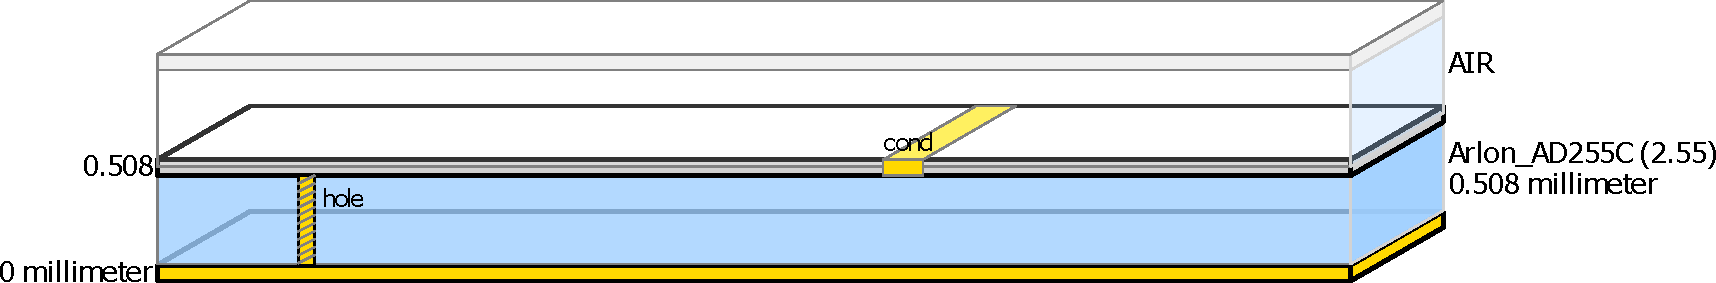
\includegraphics[width=0.9\textwidth]{matching_substrate.pdf}
    \caption{Подложка}
    \label{fig:matching_substrate}
\end{figure}

\subsection{Модель на идеальных линиях передачи}

Соберём моделируемую схему на идеальных линиях передачи (Рис. \ref{fig:matching_ideal_schematic_1}). Для расчёта электрических длин TLSC и TLIN воспользуемся встроенным инструментом Smith Chart. Зафиксировав значения $Z_S$ и $Z_L$ получим, что искомые электрические длины равны $68.258$ и $125.029$ соответственно.

\begin{figure}[!ht]
    \centering
    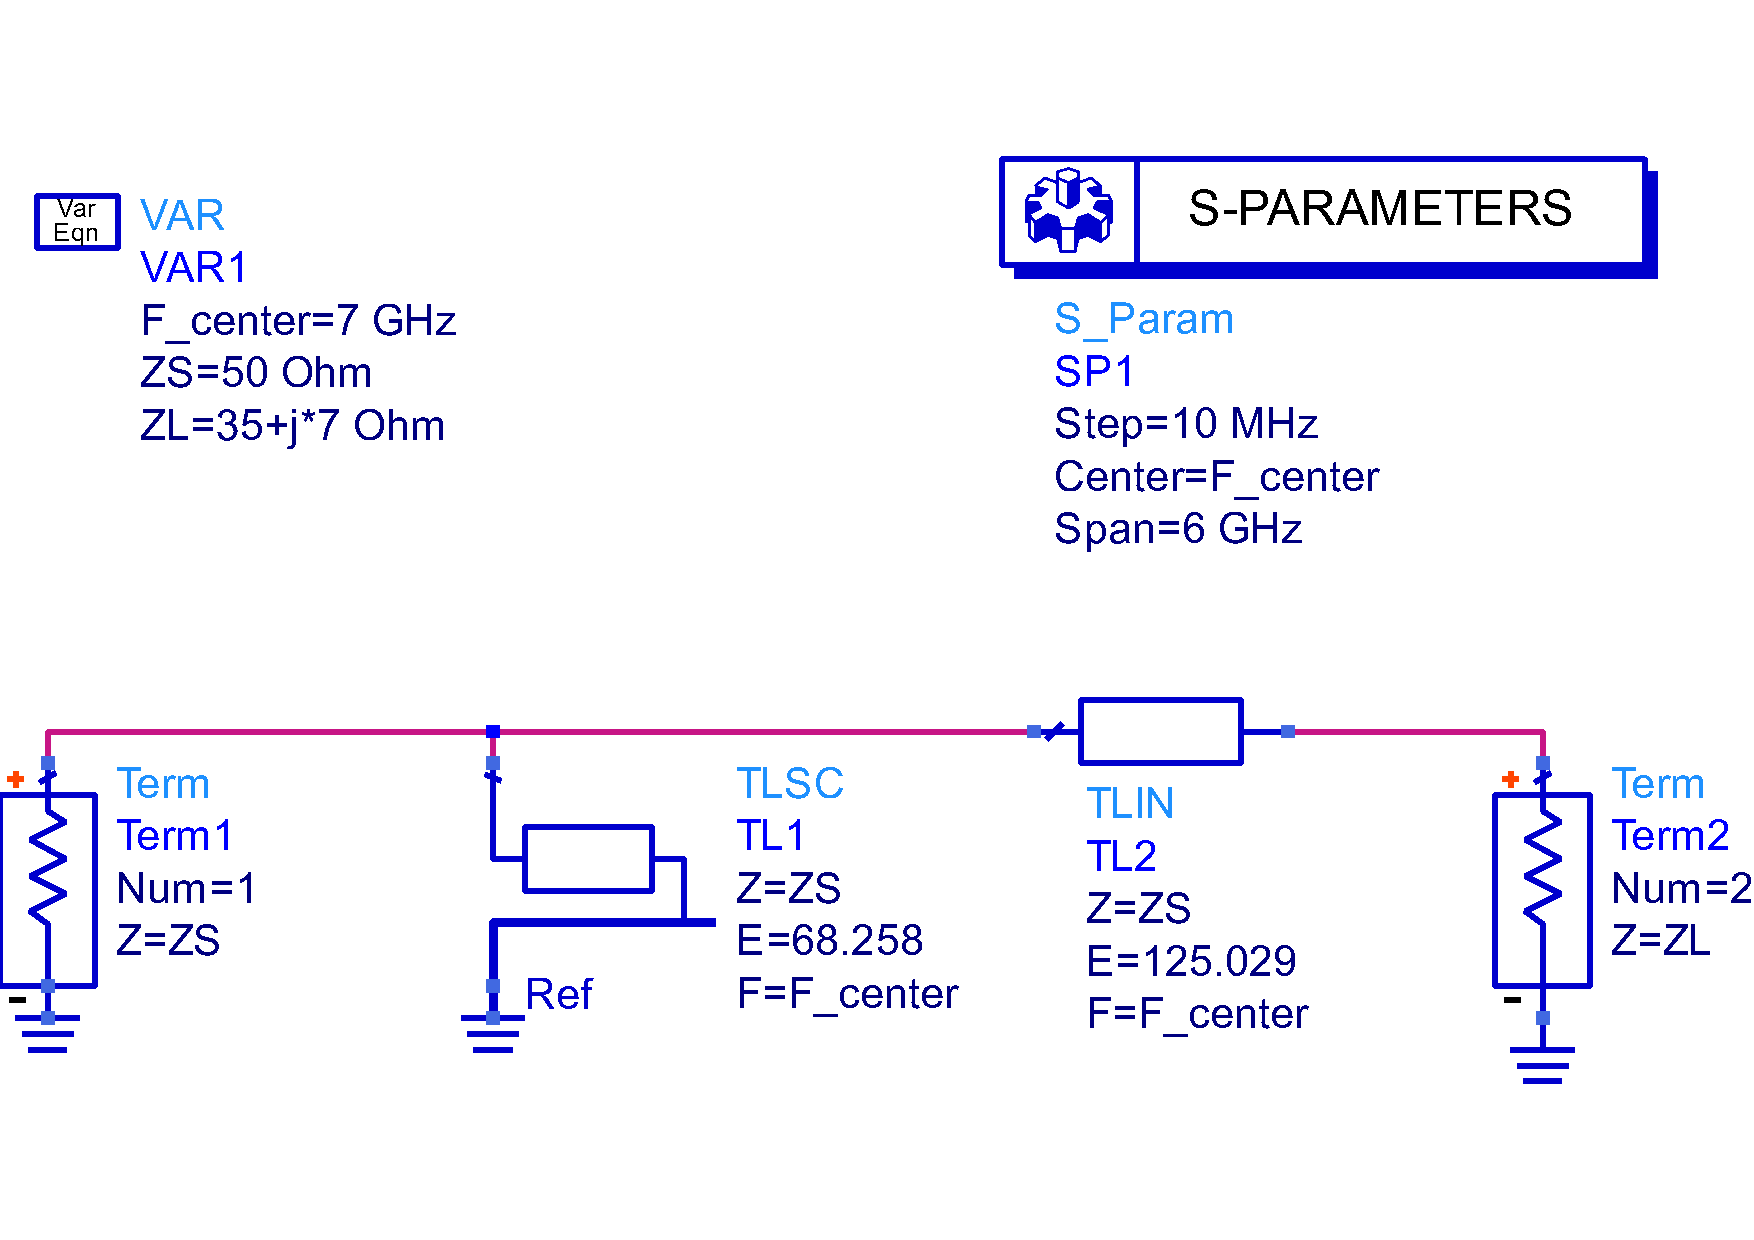
\includegraphics[width=0.8\textwidth]{matching_ideal_schematic_1.pdf}
    \caption{Моделируемая цепь на идеальных линиях передачи}
    \label{fig:matching_ideal_schematic_1}
\end{figure}

Результаты моделирования можно увидеть на рис. \ref{fig:matching_ideal_data_1_freq_response}.

\begin{figure}[!ht]
    \centering
    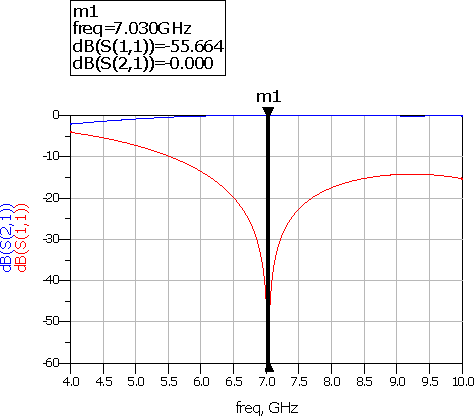
\includegraphics[width=0.6\textwidth]{matching_ideal_data_1_freq_response.pdf}
    \caption{Результаты моделирования цепи на идеальных линиях передачи}
    \label{fig:matching_ideal_data_1_freq_response}
\end{figure}

Для наглядного представления о согласовании в заданной полосе частот выведем диаграмму Смита (Рис. \ref{fig:matching_ideal_data_1_smith_chart}) и зависимость КСВН от частоты (Рис. \ref{fig:matching_ideal_data_1_vswr}).

\begin{figure}[!ht]
    \begin{subfigure}[b]{0.45\textwidth}
        \centering
        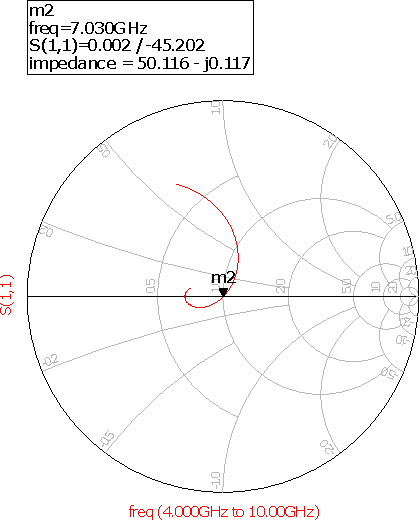
\includegraphics[width=\textwidth]{matching_ideal_data_1_smith_chart.pdf}
        \caption{}
        \label{fig:matching_ideal_data_1_smith_chart}
    \end{subfigure}
    \hfill
    \begin{subfigure}[b]{0.45\textwidth}
        \centering
        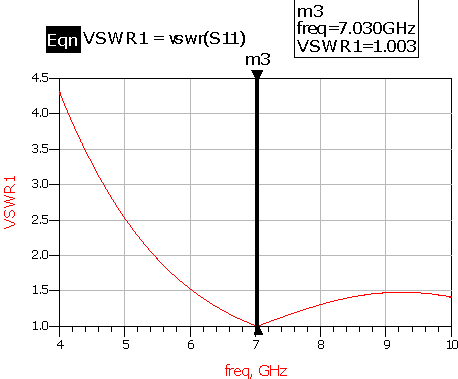
\includegraphics[width=\textwidth]{matching_ideal_data_1_vswr.pdf}
        \caption{}
        \label{fig:matching_ideal_data_1_vswr}
    \end{subfigure}
    \caption{
        a) диаграмма Смита;
        б) зависимость КСВН от частоты
    }
    \label{fig:matching_ideal_data_display_1}
\end{figure}

\subsection{Модель на схемном уровне в микрополосковом исполнении}

Для расчёта геометрических размеров нескольких видов линий передач воспользуемся инструментом LineCalc, которую можно найти по пути Tools \textrightarrow LineCalc \textrightarrow Start LineCalc.

В подокне Substrate Parameters задаём параметры подложки из технического задания, в подокне Component Parameters задаём частоту из технического задания, а в подокне Electrical "--- импеданс и электрическую длину, для которых ведётся расчёт.
После этого, нажав кнопку Synthesize, получим в подокне Physical искомые геометрические размеры.

Расчитаем таким образом размеры короткозамкнутого шлейфа и последовательного участка.
Получим $W_\text{shunt} = 1.383 \text{~мм}$, $L_\text{shunt} = 5.589 \text{~мм}$ и $W_\text{serial} = 1.383 \text{~мм}$, $L_\text{serial} = 10.238 \text{~мм}$ соответственно.

Построим моделируемую схему в микрополосковом исполнении (Рис. \ref{fig:matching_MLIN_schematic_1}).

\begin{figure}[!ht]
    \centering
    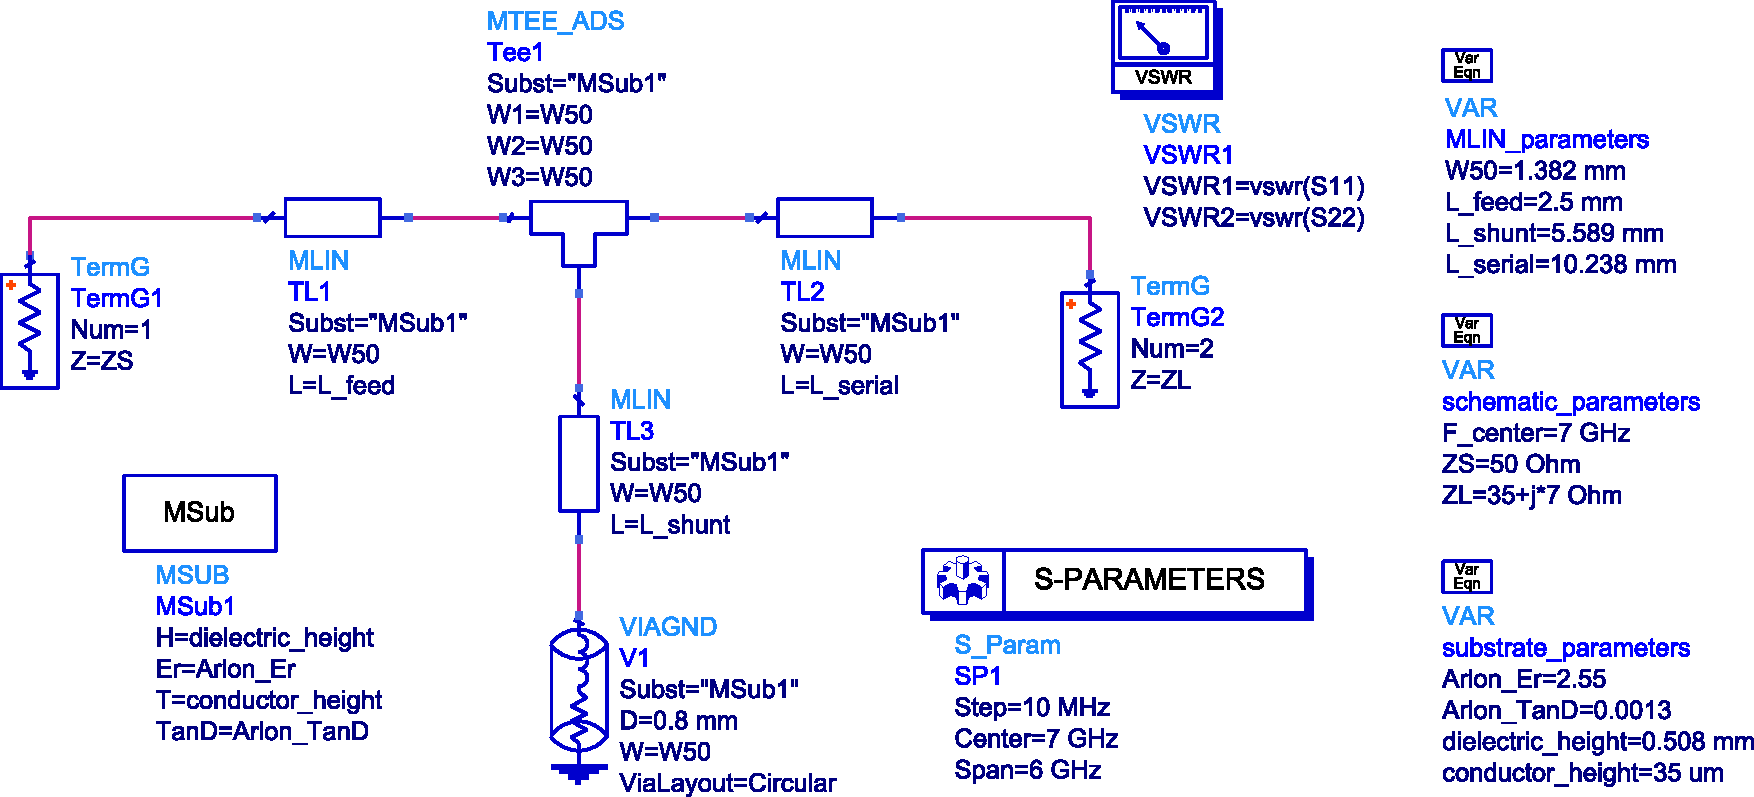
\includegraphics[width=0.8\textwidth]{matching_MLIN_schematic_1.pdf}
    \caption{Моделируемая схема в микрополосковом исполнении}
    \label{fig:matching_MLIN_schematic_1}
\end{figure}

Запустим расчёт и построим диаграмму Смита и зависимость КСВН от частоты (Рис. \ref{fig:matching_MLIN_data_display_1}).

\begin{figure}[!ht]
    \begin{subfigure}[b]{0.45\textwidth}
        \centering
        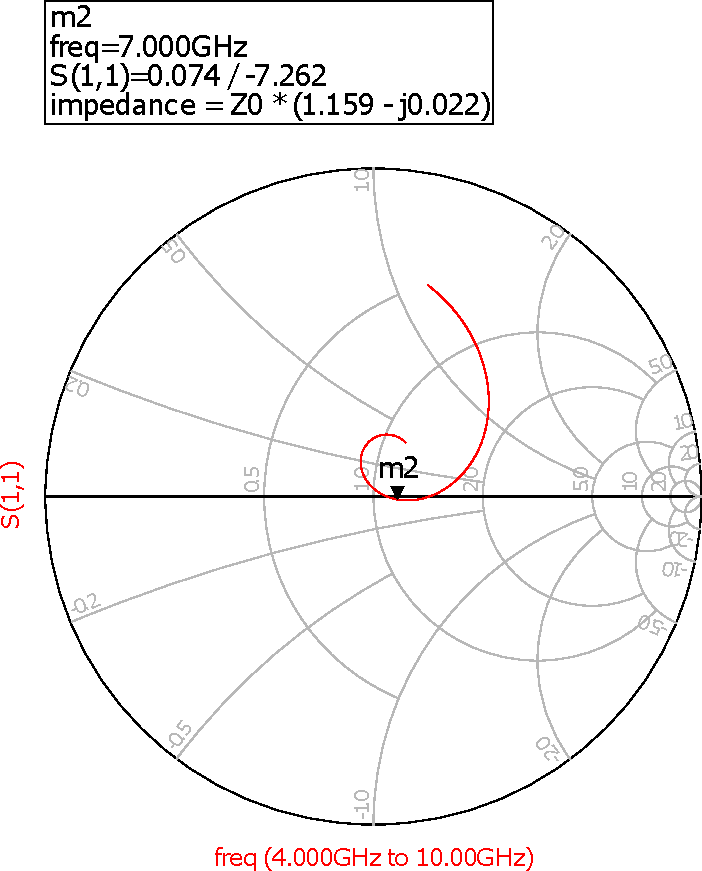
\includegraphics[width=\textwidth]{matching_MLIN_data_1_smith_chart.pdf}
        \caption{}
        \label{fig:matching_MLIN_data_1_smith_chart}
    \end{subfigure}
    \hfill
    \begin{subfigure}[b]{0.45\textwidth}
        \centering
        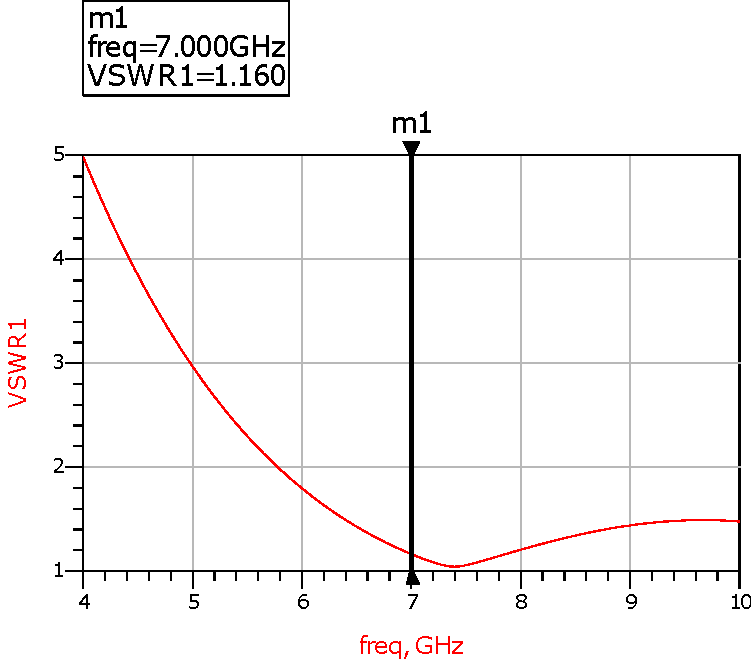
\includegraphics[width=\textwidth]{matching_MLIN_data_1_vswr.pdf}
        \caption{}
        \label{fig:matching_MLIN_data_1_vswr}
    \end{subfigure}
    \caption{
        a) диаграмма Смита;
        б) зависимость КСВН от частоты
    }
    \label{fig:matching_MLIN_data_display_1}
\end{figure}

Видно, что КСВН близко к 1 и S11 практически в центре.
Для того, чтобы окончательно довести до идеала согласование на требуемой частоте, воспользуемся инструментом Tune.
В качестве изменяемых параметров укажем $L_\text{shunt}$ и $L_\text{serial}$ для чего щёлкнем по ним левой кнопкой мыши.
Подберём оптимальный размер шага, после чего изменяя значения выбранных параметров с помощью слайдера, найдём такие, при которых обеспечивается наилучшее согласование.
Для переноса этих значений на схему, нажмём кнопку Update Schematic в окне Tune Parameters.

Итоговую схему можем увидеть на рис. \ref{fig:matching_MLIN_schematic_2}.

\begin{figure}
    \centering
    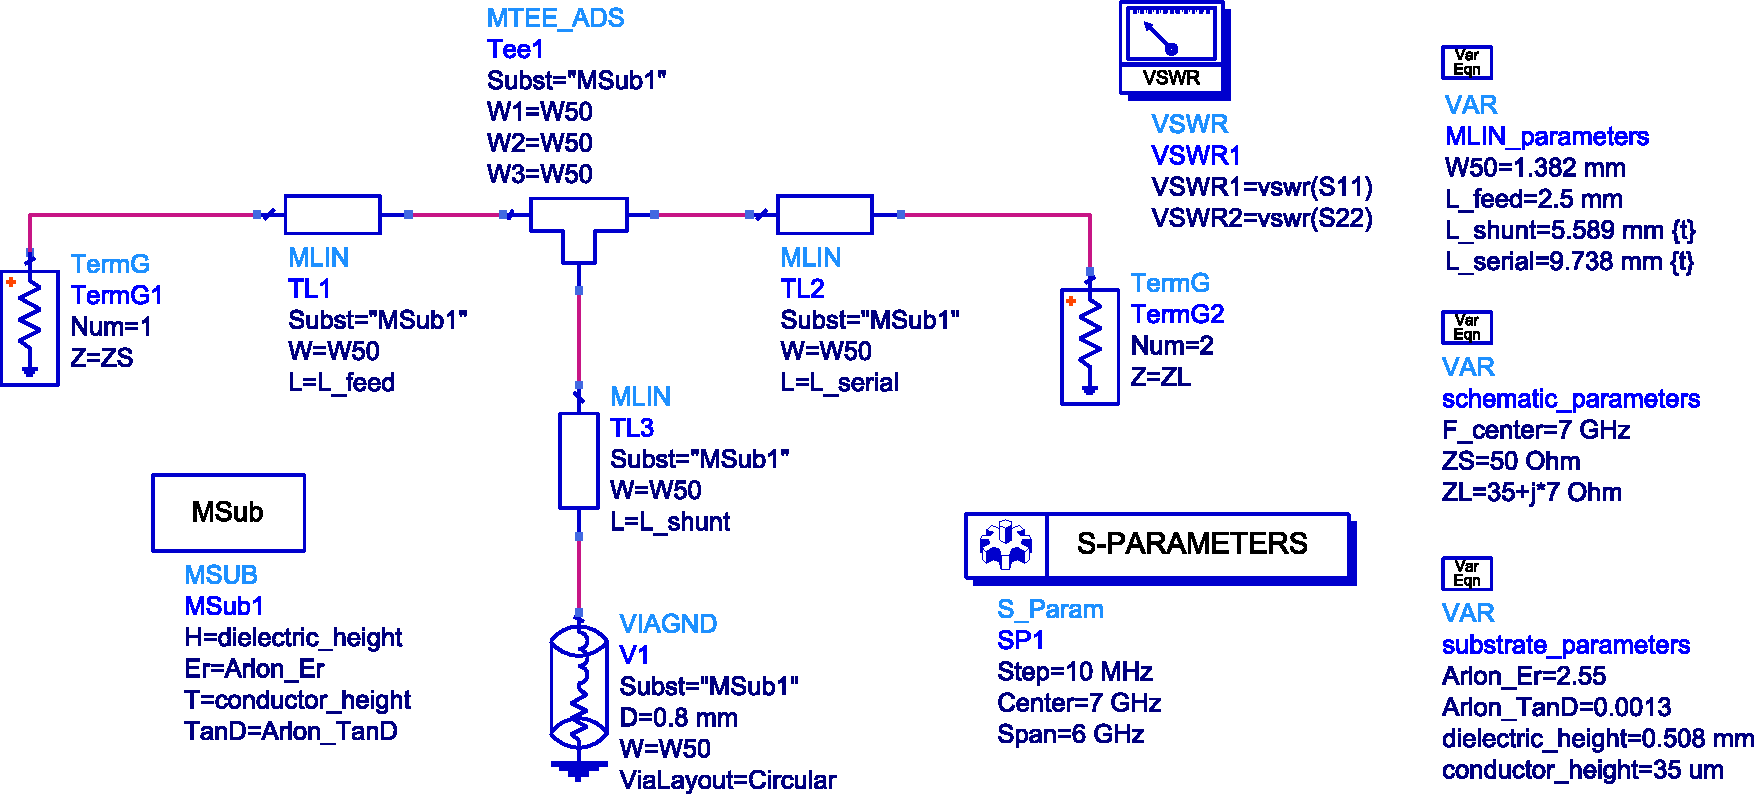
\includegraphics[width=0.6\textwidth]{matching_MLIN_schematic_2.pdf}
    \caption{Моделируемая схема в микрополосковом исполнении после применения инструмента Tune}
    \label{fig:matching_MLIN_schematic_2}
\end{figure}

\subsection{Модель на топологическом уровне}

Скопируем схему в микрополосковом исполнении в новую ячейку. Сделаем её двухуровневой, перенеся во внутренний уровень все полосковые устройства. Сделать это можно по команде Edit \textrightarrow Component \textrightarrow Create Hierarchy.

В результате получим схему верхнего уровня (Рис. \ref{fig:matching_EM_schematic}) и схему нижнего уровня (Рис. \ref{fig:matching_EM_inner_schematic}).

\begin{figure}[!ht]
    \begin{subfigure}[b]{0.6\textwidth}
        \centering
        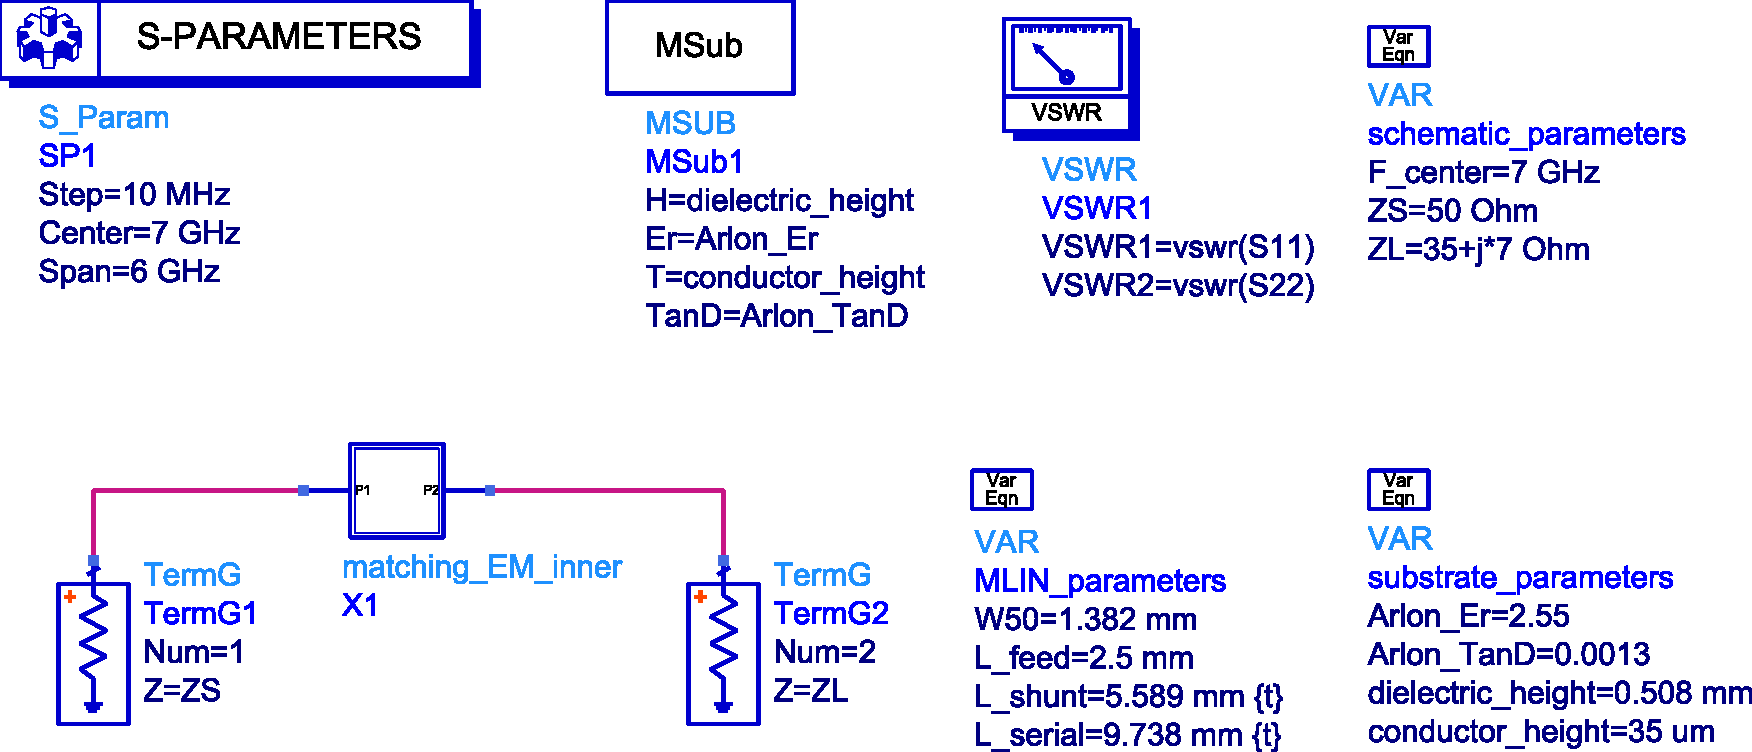
\includegraphics[width=\textwidth]{matching_EM_schematic_1.pdf}
        \caption{}
        \label{fig:matching_EM_schematic}
    \end{subfigure}
    \hfill
    \begin{subfigure}[b]{0.3\textwidth}
        \centering
        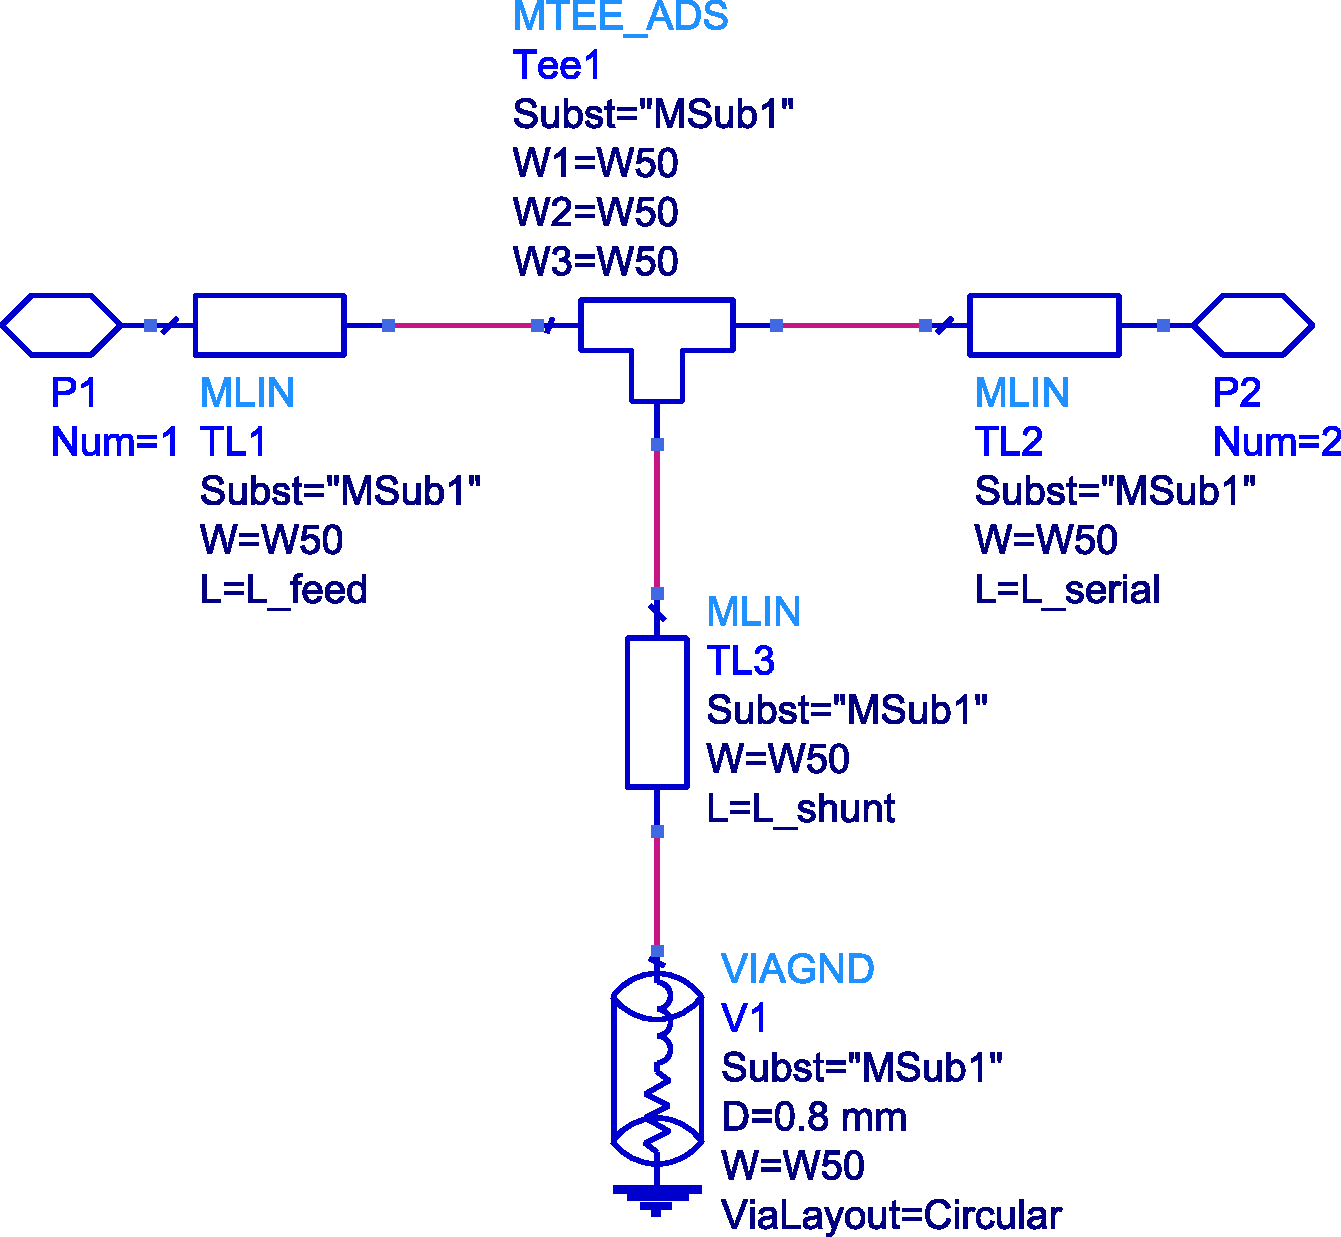
\includegraphics[width=\textwidth]{matching_EM_inner_schematic_1.pdf}
        \caption{}
        \label{fig:matching_EM_inner_schematic}
    \end{subfigure}
    \caption{
        a) внешнаяя схема;
        б) внутренняя схема
    }
    \label{fig:matching_EM_schematics}
\end{figure}

Перейдём в схему нижнего уровня. Для получения топологического представления воспользуемся функцией Layout \textrightarrow Generate/Update Layout.
Топологическое представление создано верно (Рис. \ref{fig:matching_layout_check}).

\begin{figure}[!ht]
    \centering
    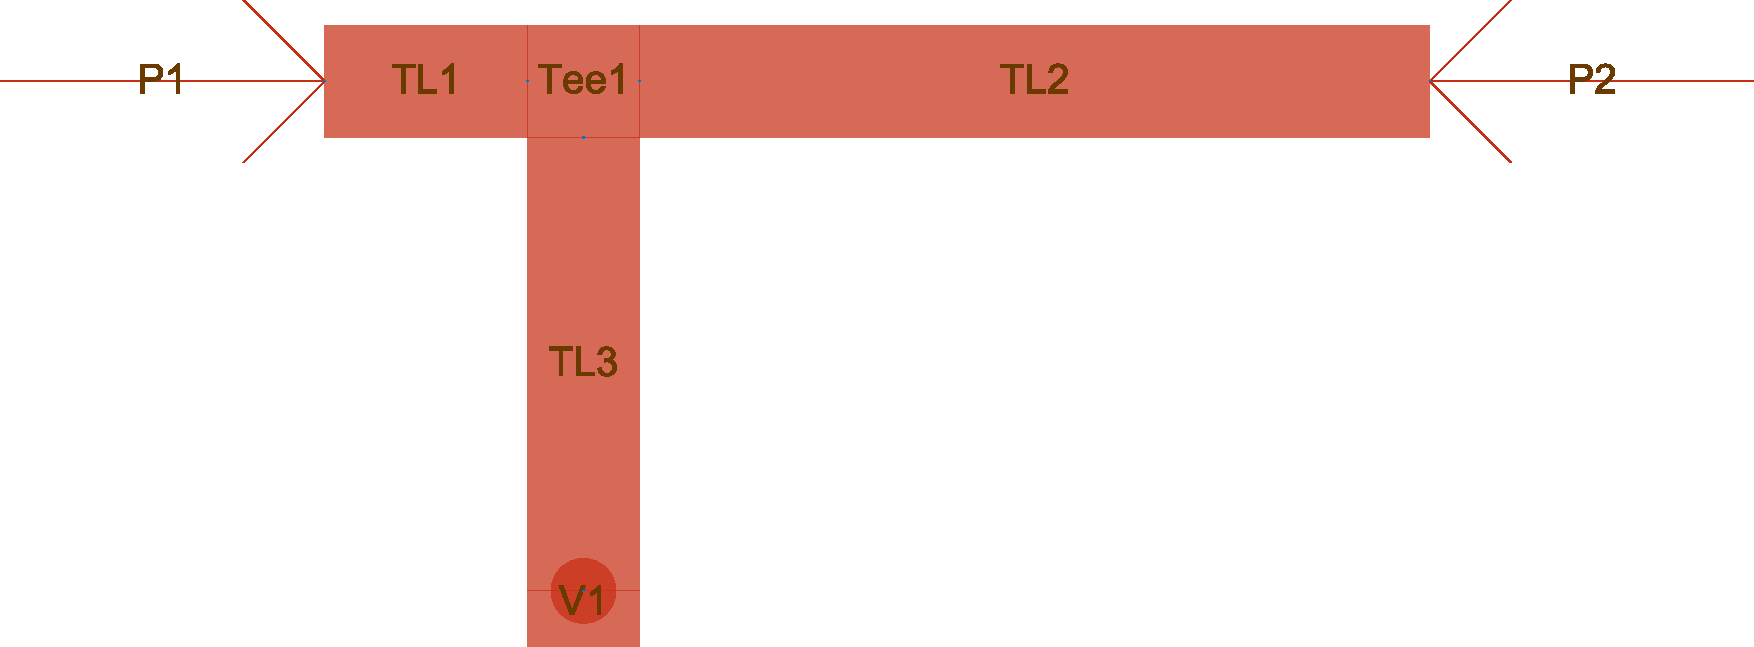
\includegraphics[width=0.8\textwidth]{matching_layout_check.pdf}
    \caption{Проверка топологического представления}
    \label{fig:matching_layout_check}
\end{figure}

Перейдём в окно File \textrightarrow Customize Pcell.
Сделаем схему параметризуемой, выбрав в выпадающем списке тип Parameterized sub network Pcell.
Также убедимся в том, что выставлены галочки напротив Support non-90 degree rotation и Support unit and database resolution for ADS 2015 and older.

В окне File \textrightarrow Cell Parameters определим параметры $W_{50}$, $L_\text{feed}$, $L_\text{shunt}$, $L_\text{serial}$.

Для EM-моделирования создадим сущность emSetup.
Это можно сделать в окне EM \textrightarrow Simulation Setting.
Определим параметры в соответствии с требованиями.
